\section{Zielsetzung}
\label{sec:Zielsetzung}
Es sollen verschiedene elektrische Schwingungen in ihre Fourierkomponenten zerlegt
werden. Im zweiten Teil des Versuchs sollen diese Funktionen durch 
Überlagerung ihrer Fourierkomponenten synthetisiert werden.


\section{Theorie}
\label{sec:Theorie}
Eine Vielzahl physikalischer Vorgänge, beispielsweise sich ausbreitende Wellen oder 
ungedämpfte Schwingungen, lassen sich durch periodische Funktionen beschreiben, die sich 
zeitlich und/oder räumlich wiederholen. Sie kehren also nach einem bestimmten Zeitraum $T$
oder einer bestimmten Distanz $D$ wieder zu ihrem Ursprungswert zurück und der Ablauf wiederholt sich.
Die am häufigsten genutzten periodischen Funktionen sind die Cosinus- und die Sinusfunktion der
Form

\begin{align}
f(t) = a \, sin \Bigl(\frac{2\pi}{T}t\Bigr) \\
\text{bzw.} \, f(t) = b \, cos \Bigl(\frac{2\pi}{T}t\Bigr),
\end{align}

mit den Amplituden $a$ und $b$ und der jeweiligen Periodendauer $T$. Nach Jean Baptiste Joseph Fourier 
lässt sich jedes periodische Phänomen der Natur durch eine Kombination dieser beschreiben,
was er in dem Fourierschen Theorem

\begin{align}
f(t) = \frac{1}{2} a_\text{0} + \sum_{n=1}^\infty \Bigl( a_\text{n} cos \Bigl( \frac{2 \pi n}{T} t \Bigr) + b_\text{n} sin \Bigl( \frac{2 \pi n}{T} t \Bigr) \Bigr)
\end{align}

formulierte. Ist die hier genannte Reihe gleichmäßig konvergent, so stellt sie eine periodische 
Funktion $f(t)$ mit der Periode $T$ dar. Die Koeffizienten $a_\text{n}$ und $b_\text{n}$ lassen sich 
nach

\begin{align}
a_\text{n} = \frac{2}{T} \int_0^T f(t) cos \Bigl( \frac{2 \pi n}{T} t \Bigr) dt \\
\text{und} \,\, b_\text{n} = \frac{2}{T} \int_0^T f(t) sin \Bigl( \frac{2 \pi n}{T} t \Bigr) dt
\end{align}

berechnen. Demnach treten durch $n \in \symbb{R}$ nur ganzzahlige Vielfache einer Grundfrequenz $\nu_\text{1}$ auf.
Werden die zur jeweiligen Oberwelle gehörigen Amplituden $a_\text{n}$ und $b_\text{n}$ als Funktion der Frequenz
aufgetragen, so ergibt sich dementsprechend ein Linienspektrum, welches in beispielhaft in Abbildung 1
zu sehen ist.

\begin{figure}
\centering
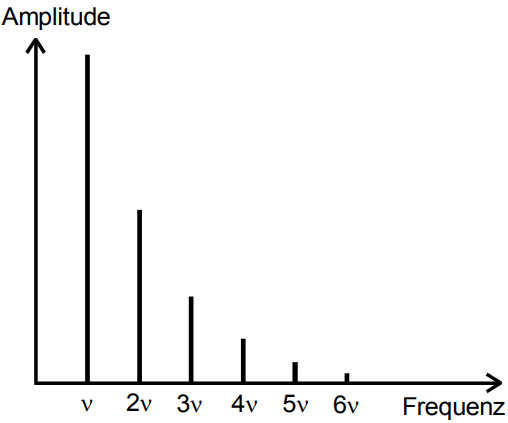
\includegraphics[scale=0.5]{frequenz.png}
\caption{Beispielhafte Amplituden einer periodischen Schwingung als Funktion der Frequenz in einem Frequenzspektrum mit der Grundfrequenz $\nu_\text{1}$ \cite[S. 271]{sample}}.
\label{fig:frequenz}
\end{figure}

Besitzt eine periodische Funktion $f(t)$ eine unstetige Stelle $t_\text{0}$, so lässt sich ein
Überschwingen beobachten, da die Funktion an der Stelle nicht approximiert werden kann. Mit wachsendem $n$ bleibt dennoch
eine endliche Abweichung der Reihe von der eigentlichen Funktion. Dies wird als Gibbsches Phänomen bezeichnet.

Mithilfe der Fourier-Transformation
\begin{align}
g(\nu) = \int_{-\infty}^\infty f(t) e^{i \nu t} dt
\end{align}
kann das gesamte Frequenzspektrum einer zeitabhängigen Funktion
unabhängig von ihrer Periodizität bestimmt werden.
Bei Funktionen die keine Periodizität aufweisen ergibt sich 
im Gegensatz zu einem Linienspektrum ein kontinuierliches Spektrum an Frequenzen, sodass bei der noch folgenden
Fourier-Analyse Nebenmaxima ausgebildet werden, da es nicht möglich ist, einen unendlich
großen Zeitraum zu betrachten. Diese werden jedoch vernachlässigt.
